\chapter{Results}
\label{chap:results}

\section{Chapter Overview}
\label{sec:results-overview}

This chapter reports the empirical results of the project: the final dataset, training behaviour, objective test-set evaluation, exported model artefacts, and plugin runtime observations. Broader interpretation is left to Chapter~5.

The chapter draws on the completed LSTM and GRU training runs, the exported JSON model files, and the final plugin tests in digital audio workstation environments. Error-to-Signal Ratio (ESR) is the primary objective accuracy metric, with SNR, correlation, RMSE, and MAE as supporting measures. Informal listening observations appear only as practical notes from deployment, not as a substitute for formal perceptual evaluation.

\section{Dataset and Experimental Artefacts}
\label{sec:dataset-and-experimental-artefacts}

The final dataset consisted of matched dry input and Boss DS-1 target recordings, divided into training, validation, and test splits and recorded at 44.1 kHz. Files were organised as paired mono input and target WAVs, which let the recurrent models learn a direct sample-level mapping from the dry guitar signal to the processed DS-1 output.

The DS-1 pedal setting and recording signal chain are documented in Appendix A. This chapter focuses on the measured dataset properties and model outcomes rather than repeating the recording methodology.

\begin{table}[htbp]
  \centering
  \caption{Dataset summary}
  \label{tab:dataset-summary}
  \resizebox{\linewidth}{!}{%
    \begin{tabular}{llrrrrr}
      \toprule
      \textbf{Split} & \textbf{Signal} & \textbf{Sample rate} & \textbf{Samples} & \textbf{Duration} & \textbf{RMS} & \textbf{Peak absolute value} \\
      \midrule
      Training & Input & 44.1 kHz & 14,994,001 & 340.00 s & 0.069594 & 0.550920 \\
      Training & Target & 44.1 kHz & 14,994,001 & 340.00 s & 0.089206 & 0.432600 \\
      Validation & Input & 44.1 kHz & 2,251,753 & 51.06 s & 0.066855 & 0.552324 \\
      Validation & Target & 44.1 kHz & 2,251,753 & 51.06 s & 0.084724 & 0.384716 \\
      Test & Input & 44.1 kHz & 2,646,001 & 60.00 s & 0.102890 & 0.565722 \\
      Test & Target & 44.1 kHz & 2,646,001 & 60.00 s & 0.115847 & 0.394543 \\
      \bottomrule
    \end{tabular}%
  }
\end{table}

The training split was substantially longer than the validation and test splits. The held-out test split provided a separate 60-second evaluation signal that was never used for model fitting, with input and target files aligned as paired recordings so that objective metrics could be computed directly from the difference between the model output and the recorded DS-1 target waveform.

\section{Training Behaviour}
\label{sec:training-behaviour}

Both recurrent models were trained with the same pipeline so that the LSTM and GRU could be compared under matched conditions: Adam optimiser, an initial learning rate of 0.005, weight decay of \(1 \times 10^{-4}\), and a validation-based learning-rate scheduler. The loss combined pre-emphasised ESR and DC terms using \(0.75 \times \mathrm{ESRPre} + 0.25 \times \mathrm{DC}\).

Figure~\ref{fig:loss_curves} shows the training and validation loss curves for both models. The LSTM kept improving for longer, reaching its best validation result at epoch 284. The GRU peaked at epoch 86 and stopped after a shorter run. So the GRU converged faster, but the LSTM ended up with the lower validation loss.

\begin{table}[htbp]
  \centering
  \caption{Training behaviour summary for the LSTM and GRU models.}
  \label{tab:training_behaviour}
  \begin{tabular}{lrrrr}
    \hline
    Model & Epochs Run & Best Epoch & Best Val. Loss & Final Train Loss \\
    \hline
    LSTM & 336 & 284 & 0.023025 & 0.021342 \\
    GRU  & 138 & 86  & 0.037394 & 0.027822 \\
    \hline
  \end{tabular}
\end{table}

Both models stopped early. The LSTM ran for 336 epochs and reached the lower best-validation loss; the GRU ran for 138 and hit its stopping condition much sooner. Looking at the curves, the GRU pulled ahead at the start of training but never caught the LSTM's eventual validation performance.

\begin{table}[htbp]
  \centering
  \caption{Validation behaviour after the best checkpoint.}
  \label{tab:validation_behaviour}
  \begin{tabular}{lrrr}
    \hline
    Model & Final Val. Loss & Generalisation Gap & Post-Best Epochs \\
    \hline
    LSTM & 0.023741 & 0.001905 & 52 \\
    GRU  & 0.044003 & 0.003760 & 52 \\
    \hline
  \end{tabular}
\end{table}

Both models continued for 52 epochs past their best validation checkpoint before stopping. The LSTM had the smaller generalisation gap at its best epoch; the GRU showed a wider gap between training and validation loss, which is one reason to report from the best-validation checkpoint rather than the final epoch.

\begin{figure}[htbp]
  \centering
  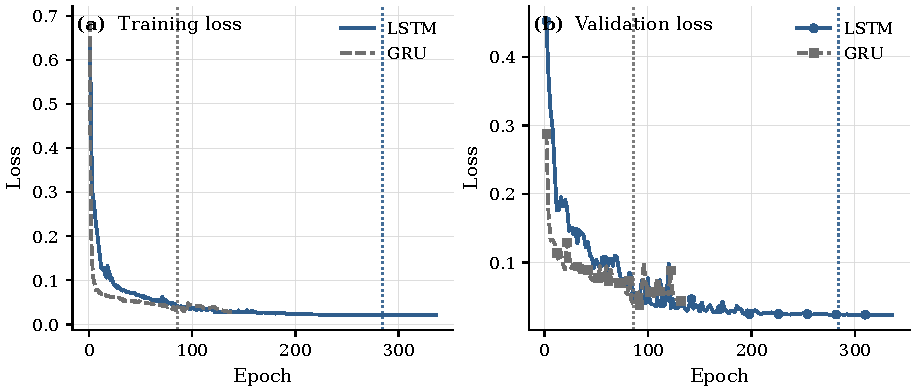
\includegraphics[width=\textwidth]{images/figures/fig_4_1_loss_curves.pdf}
  \caption[Training and validation loss curves]{Training and validation loss curves for the LSTM and GRU models. Full-resolution curves are provided in Appendix~C.}
  \label{fig:loss_curves}
\end{figure}

\begin{figure}[htbp]
  \centering
  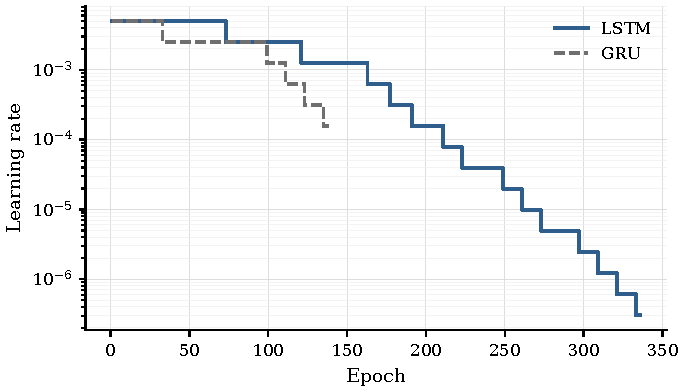
\includegraphics[width=\textwidth]{images/figures/fig_4_2_learning_rate_schedule.pdf}
  \caption[Learning-rate schedule]{Learning-rate schedule during LSTM and GRU training.}
  \label{fig:learning_rate}
\end{figure}

\section{Objective Test-Set Evaluation}
\label{sec:objective-test-set-evaluation}

The held-out test set was used for objective comparison between each model output and the recorded Boss DS-1 target. The best-validation checkpoint is treated as the primary model for comparison, since it reflects the state selected by validation performance rather than the final training epoch.

ESR is the main accuracy metric because it measures model error energy relative to target signal energy. SNR and correlation play supporting roles. SNR here should be read as error-relative (the ``noise'' is prediction error, not noise in the recording chain), and correlation gives a broad measure of waveform similarity rather than a perceptual quality score.

\begin{table}[htbp]
  \centering
  \caption{Objective test-set metrics}
  \label{tab:objective-test-set-metrics}
  \resizebox{\linewidth}{!}{%
    \begin{tabular}{llrrrrrr}
      \toprule
      \textbf{Model} & \textbf{Checkpoint} & \textbf{MSE} & \textbf{RMSE} & \textbf{MAE} & \textbf{ESR} & \textbf{SNR} & \textbf{Correlation} \\
      \midrule
      LSTM & Best validation & 0.00028735 & 0.016951 & 0.011324 & 0.021411 & 16.69 dB & 0.989516 \\
      LSTM & Final & 0.00028802 & 0.016971 & 0.011265 & 0.021462 & 16.68 dB & 0.989433 \\
      GRU & Best validation & 0.00048230 & 0.021961 & 0.015448 & 0.035938 & 14.44 dB & 0.981887 \\
      GRU & Final & 0.00050546 & 0.022482 & 0.015094 & 0.037663 & 14.24 dB & 0.981595 \\
      \bottomrule
    \end{tabular}%
  }
\end{table}

The LSTM produced the lowest test-set ESR at 0.021411, against 0.035938 for the GRU at its best-validation checkpoint. The supporting metrics tell the same story: lower RMSE and MAE, higher error-relative SNR, and higher waveform correlation for the LSTM on the held-out test material.

The two checkpoints reinforce the case for validation-selected reporting. The LSTM's final checkpoint sat very close to its best-validation result, with only a small uptick in ESR. The GRU showed a larger gap between the two, suggesting its final state was less favourable than the validation-selected checkpoint.

\begin{table}[htbp]
  \centering
  \caption{Best-validation versus final-checkpoint ESR}
  \label{tab:best-validation-versus-final-checkpoint-esr}
  \begin{tabular}{lrrr}
    \toprule
    \textbf{Model} & \textbf{Best-validation ESR} & \textbf{Final ESR} & \textbf{Difference} \\
    \midrule
    LSTM & 0.021411 & 0.021462 & +0.000051 \\
    GRU & 0.035938 & 0.037663 & +0.001725 \\
    \bottomrule
  \end{tabular}
\end{table}

Figure 4.3 shows an example waveform comparison between the target DS-1 recording and the model outputs, and Figure 4.4 shows a spectrogram comparison for the same region. They illustrate the structure of the model outputs and the residual differences; the numerical metrics in Table 4.4 remain the primary results.

\begin{figure}[htbp]
  \centering
  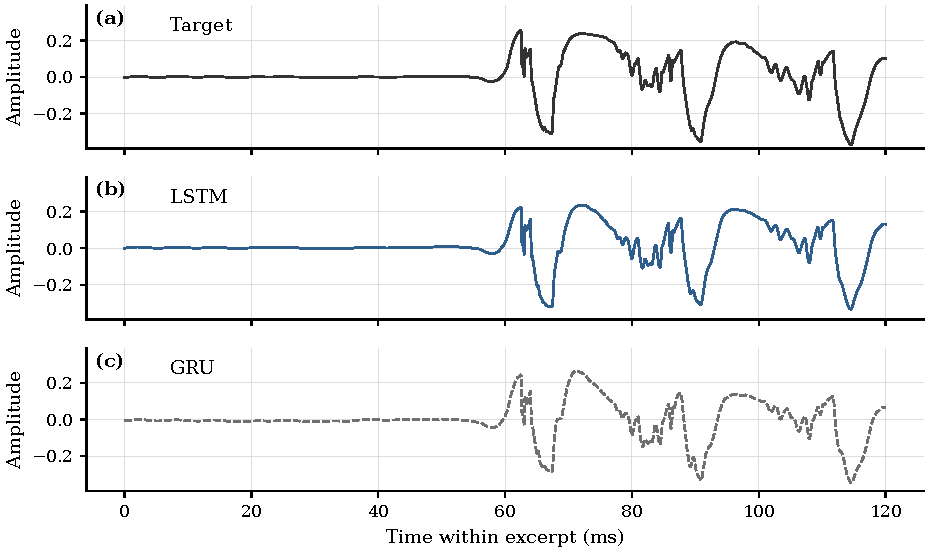
\includegraphics[width=\textwidth]{images/figures/fig_4_3_waveform_comparison.pdf}
  \caption[Test-set waveform comparison]{Example test-set waveform comparison}
  \label{fig:example-test-set-waveform-comparison}
\end{figure}

\begin{figure}[htbp]
  \centering
  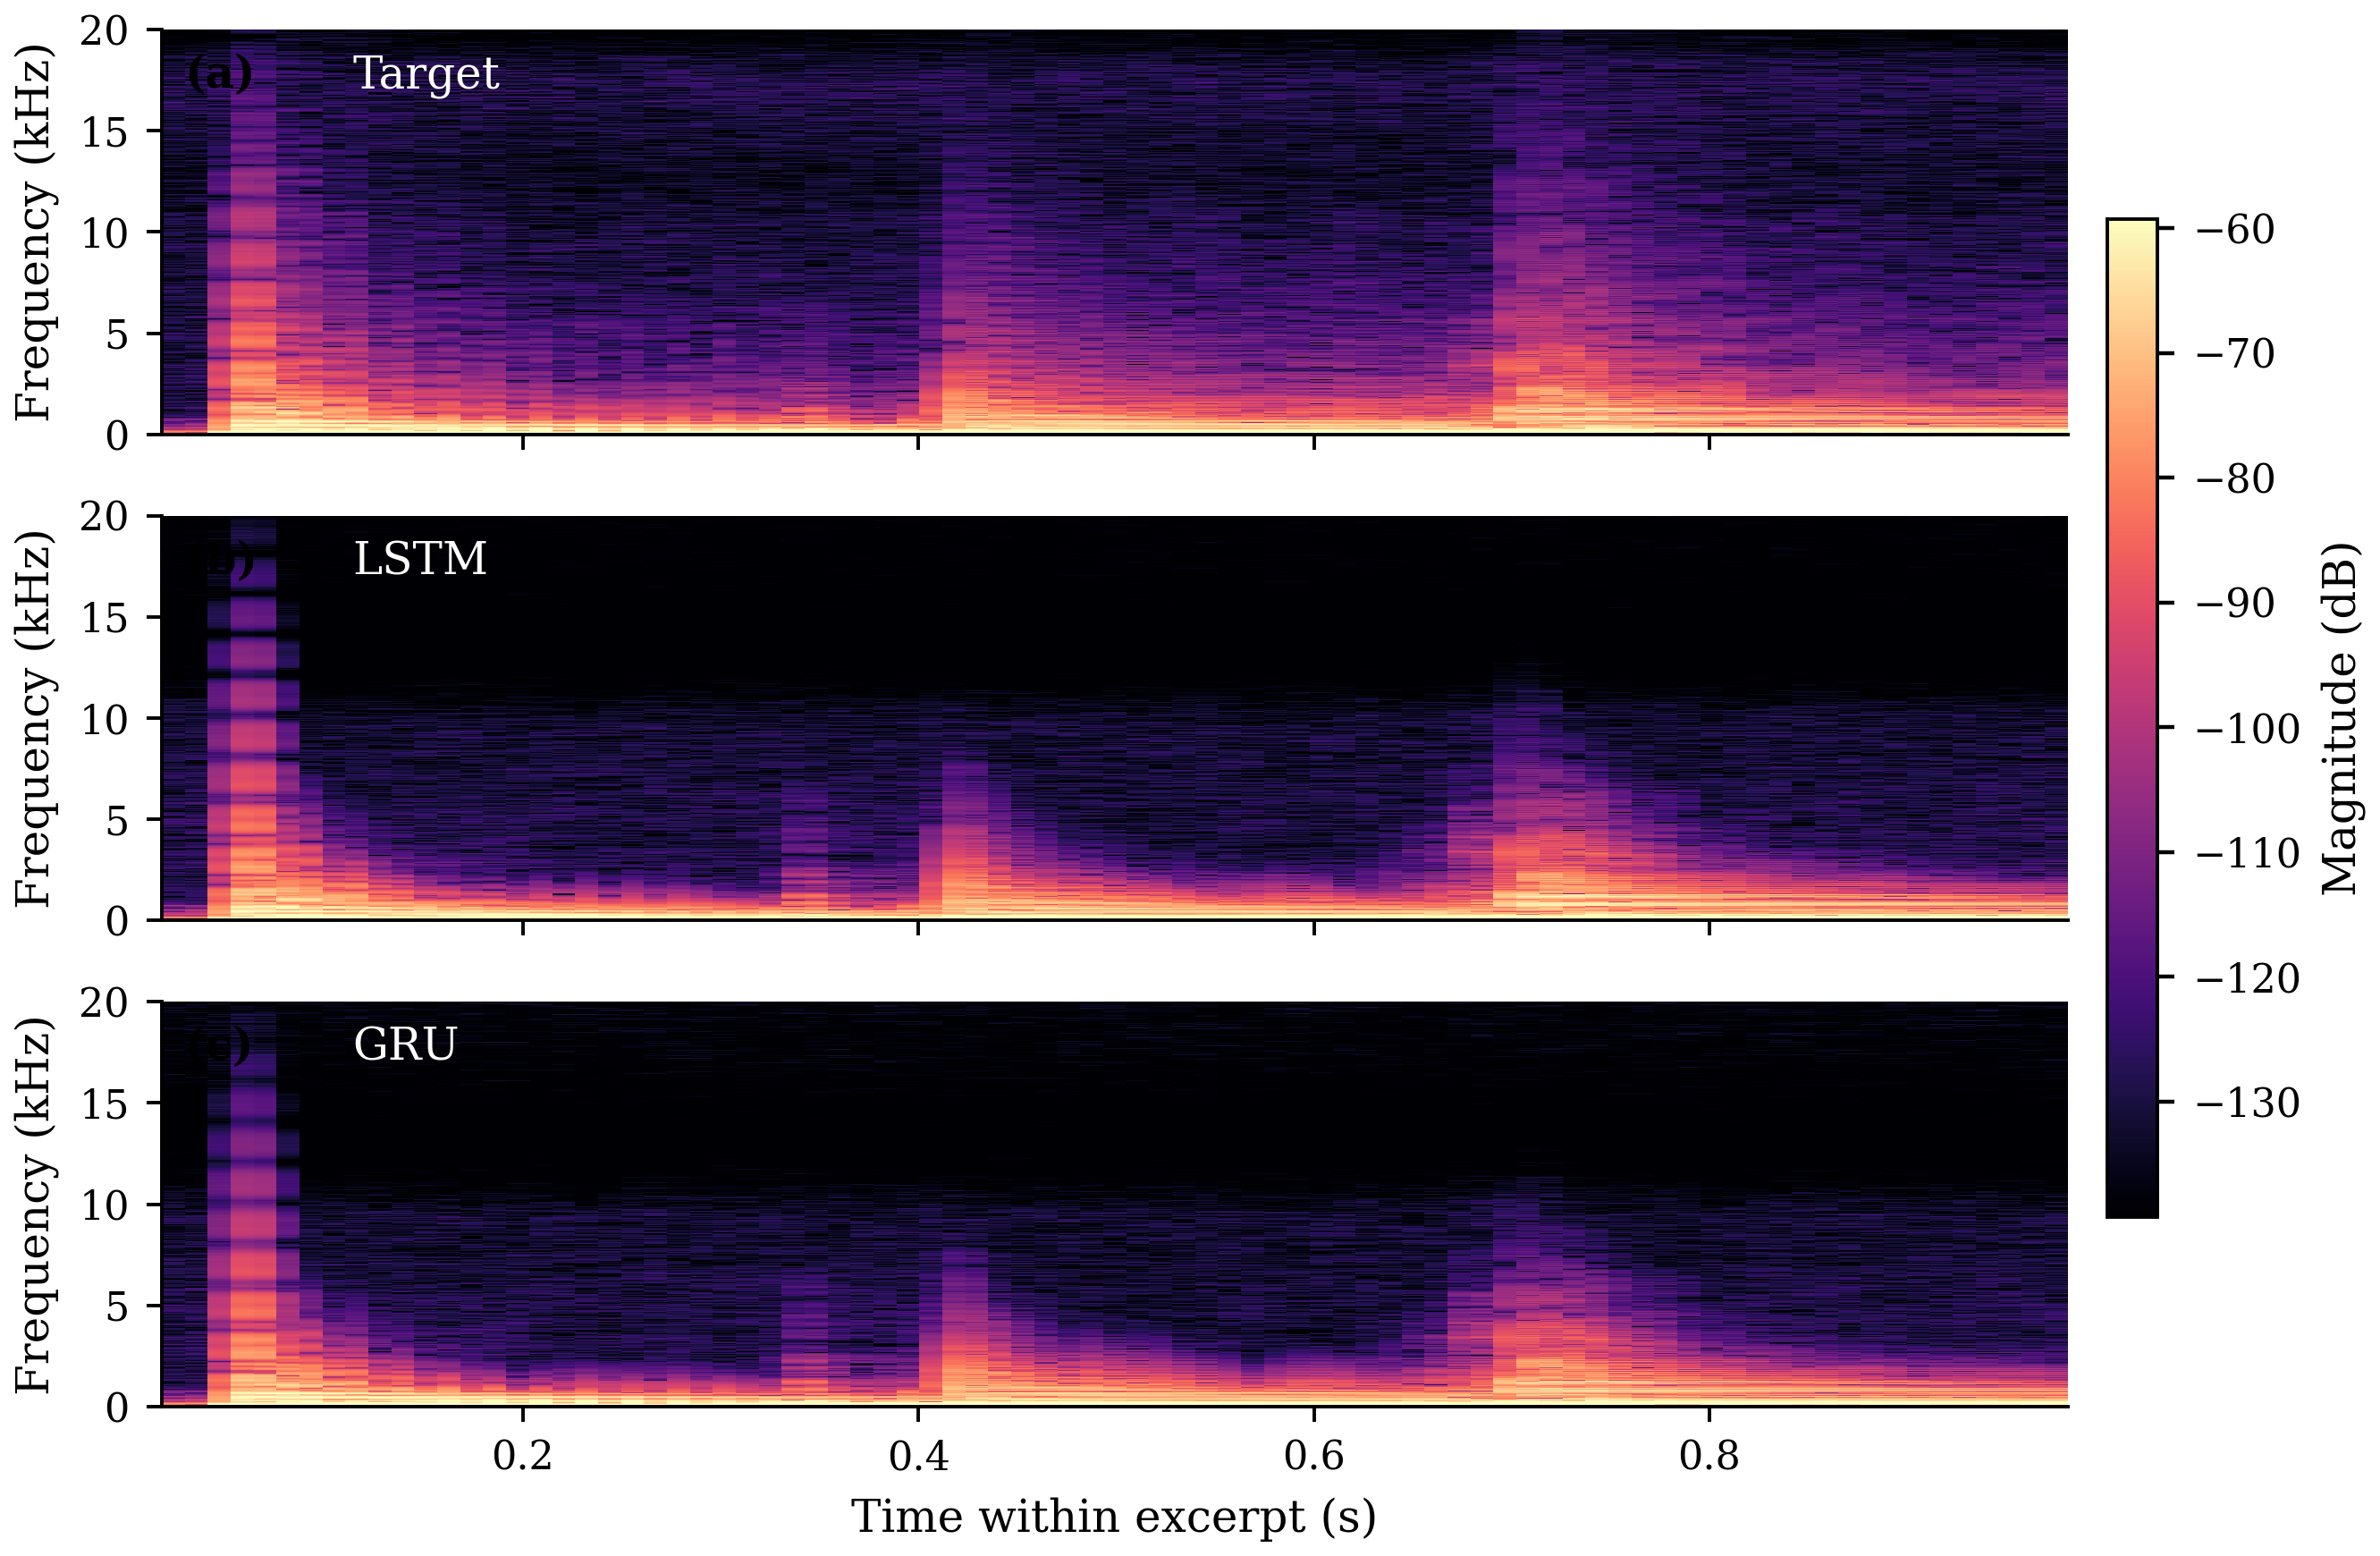
\includegraphics[width=\textwidth]{images/figures/fig_4_4_spectrogram_comparison.png}
  \caption[Test-set spectrogram comparison]{Example spectrogram comparison}
  \label{fig:example-spectrogram-comparison}
\end{figure}

Informal monitoring during plugin testing suggested both models produced broadly usable outputs, with the LSTM sounding a little closer on high-frequency detail. No controlled listening test was run, so these observations are practical notes only, not formal perceptual evidence.

\section{Architecture and Parameter Comparison}
\label{sec:architecture-and-parameter-comparison}

Both models shared the same compact, plugin-compatible recurrent architecture: a mono \texttt{SimpleRNN} with one recurrent layer, hidden size 24, a dense output stage, and a skip connection. The only architectural change between them was the recurrent cell type (LSTM in one, GRU in the other). Hidden size was held at 24 for both so the architectures could be evaluated under the same deployment constraint; the implications of that constraint are picked up in Chapter~5.

\begin{table}[htbp]
  \centering
  \caption{Shared architecture settings used by both recurrent models.}
  \label{tab:shared_architecture}
  \begin{tabular}{lr}
    \hline
    Setting & Value \\
    \hline
    Model wrapper & \texttt{SimpleRNN} \\
    Input size & 1 \\
    Output size & 1 \\
    Hidden size & 24 \\
    Recurrent layers & 1 \\
    Skip connection & Enabled \\
    Bias & Enabled \\
    \hline
  \end{tabular}
\end{table}

Table~\ref{tab:shared_architecture} lists the shared settings used by both exported models, matching the plugin-compatible format from the deployment stage. The recurrent unit type and resulting parameter count are shown separately in Table~\ref{tab:parameter_comparison}.

\begin{table}[htbp]
  \centering
  \caption{Parameter comparison between the matched LSTM and GRU models.}
  \label{tab:parameter_comparison}
  \begin{tabular}{llrr}
    \hline
    Model & Unit Type & Parameters & Difference from LSTM \\
    \hline
    LSTM & LSTM & 2,617 & -- \\
    GRU  & GRU  & 1,969 & -648 \\
    \hline
  \end{tabular}
\end{table}

Under the matched hidden-size-24 configuration the GRU used 648 fewer parameters than the LSTM. That gap is expected: the LSTM cell carries four gate groups against the GRU's three. So the GRU was the smaller model, while the LSTM produced the lower objective test-set error reported in Section~\ref{sec:objective-test-set-evaluation}.

\begin{figure}[htbp]
  \centering
  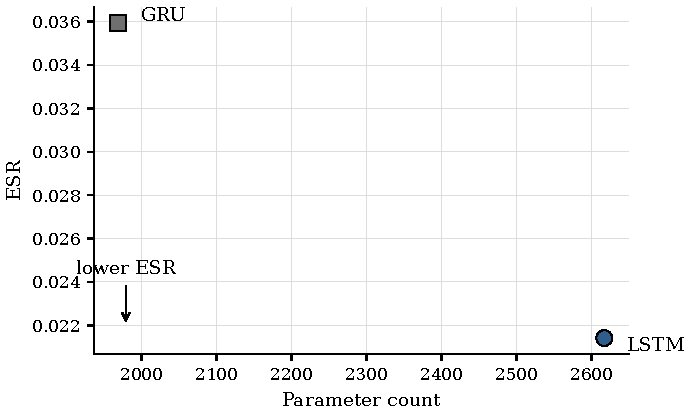
\includegraphics[width=0.9\textwidth]{images/figures/fig_4_5_accuracy_efficiency.pdf}
  \caption[Accuracy--efficiency comparison]{Accuracy--efficiency comparison between the matched LSTM and GRU models.}
  \label{fig:accuracy-efficiency-comparison}
\end{figure}

\section{Exported Model Artefacts}
\label{sec:exported-model-artefacts}

Both trained models were exported as JSON files for the C++ plugin. The artefacts include the final model and the best-validation checkpoint for each architecture; the best-validation files were used for the primary comparison because they correspond to the checkpoint selected by validation performance.

\begin{table}[htbp]
  \centering
  \caption{Exported model artefacts}
  \label{tab:exported-model-artefacts}
  \resizebox{\linewidth}{!}{%
    \begin{tabular}{llll}
      \toprule
      \textbf{Model} & \textbf{Artefact} & \textbf{Path} & \textbf{Approximate size} \\
      \midrule
      LSTM & Best-validation model & \texttt{Results/ds1-LSTM/model\_best.json} & 0.055 MB \\
      LSTM & Final model & \texttt{Results/ds1-LSTM/model.json} & 0.055 MB \\
      GRU & Best-validation model & \texttt{Results/ds1-GRU/model\_best.json} & 0.041 MB \\
      GRU & Final model & \texttt{Results/ds1-GRU/model.json} & 0.041 MB \\
      \bottomrule
    \end{tabular}%
  }
\end{table}

The plugin-side model loader was constrained to accept the configuration used in this project: \texttt{SimpleRNN}, mono input and output, one recurrent layer, hidden size 24, LSTM or GRU cell type, and a valid skip-connection setting. Under those constraints, the exported LSTM and GRU models loaded without issue during plugin testing, and no model-loading failures were observed in the final tests.

\section{Plugin Runtime Observations}
\label{sec:plugin-runtime-observations}

The exported models were tested in the deployed JUCE and RTNeural plugin, built as VST3 and AU. Runtime testing took place in Ableton Live 12 and Cubase 12 on an M2 Max MacBook Pro with 32 GB unified memory, running macOS Tahoe. Since the trained models operate at 44.1~kHz, runtime validation here is limited to 44.1~kHz host sessions.

The plugin exposed the controls required for the research artefact (Drive, Level, Bypass, and Model selection). Both LSTM and GRU models loaded correctly and could be selected from within the plugin. No model-loading errors, control-related glitches, or audible artefacts during knob movement turned up in the final tests.

Figure~\ref{fig:plugin-ui-ableton-results} shows the deployed plugin loaded in Ableton Live 12 during the final runtime tests, documenting the research artefact as it appeared in a representative host.

\begin{figure}[htbp]
  \centering
  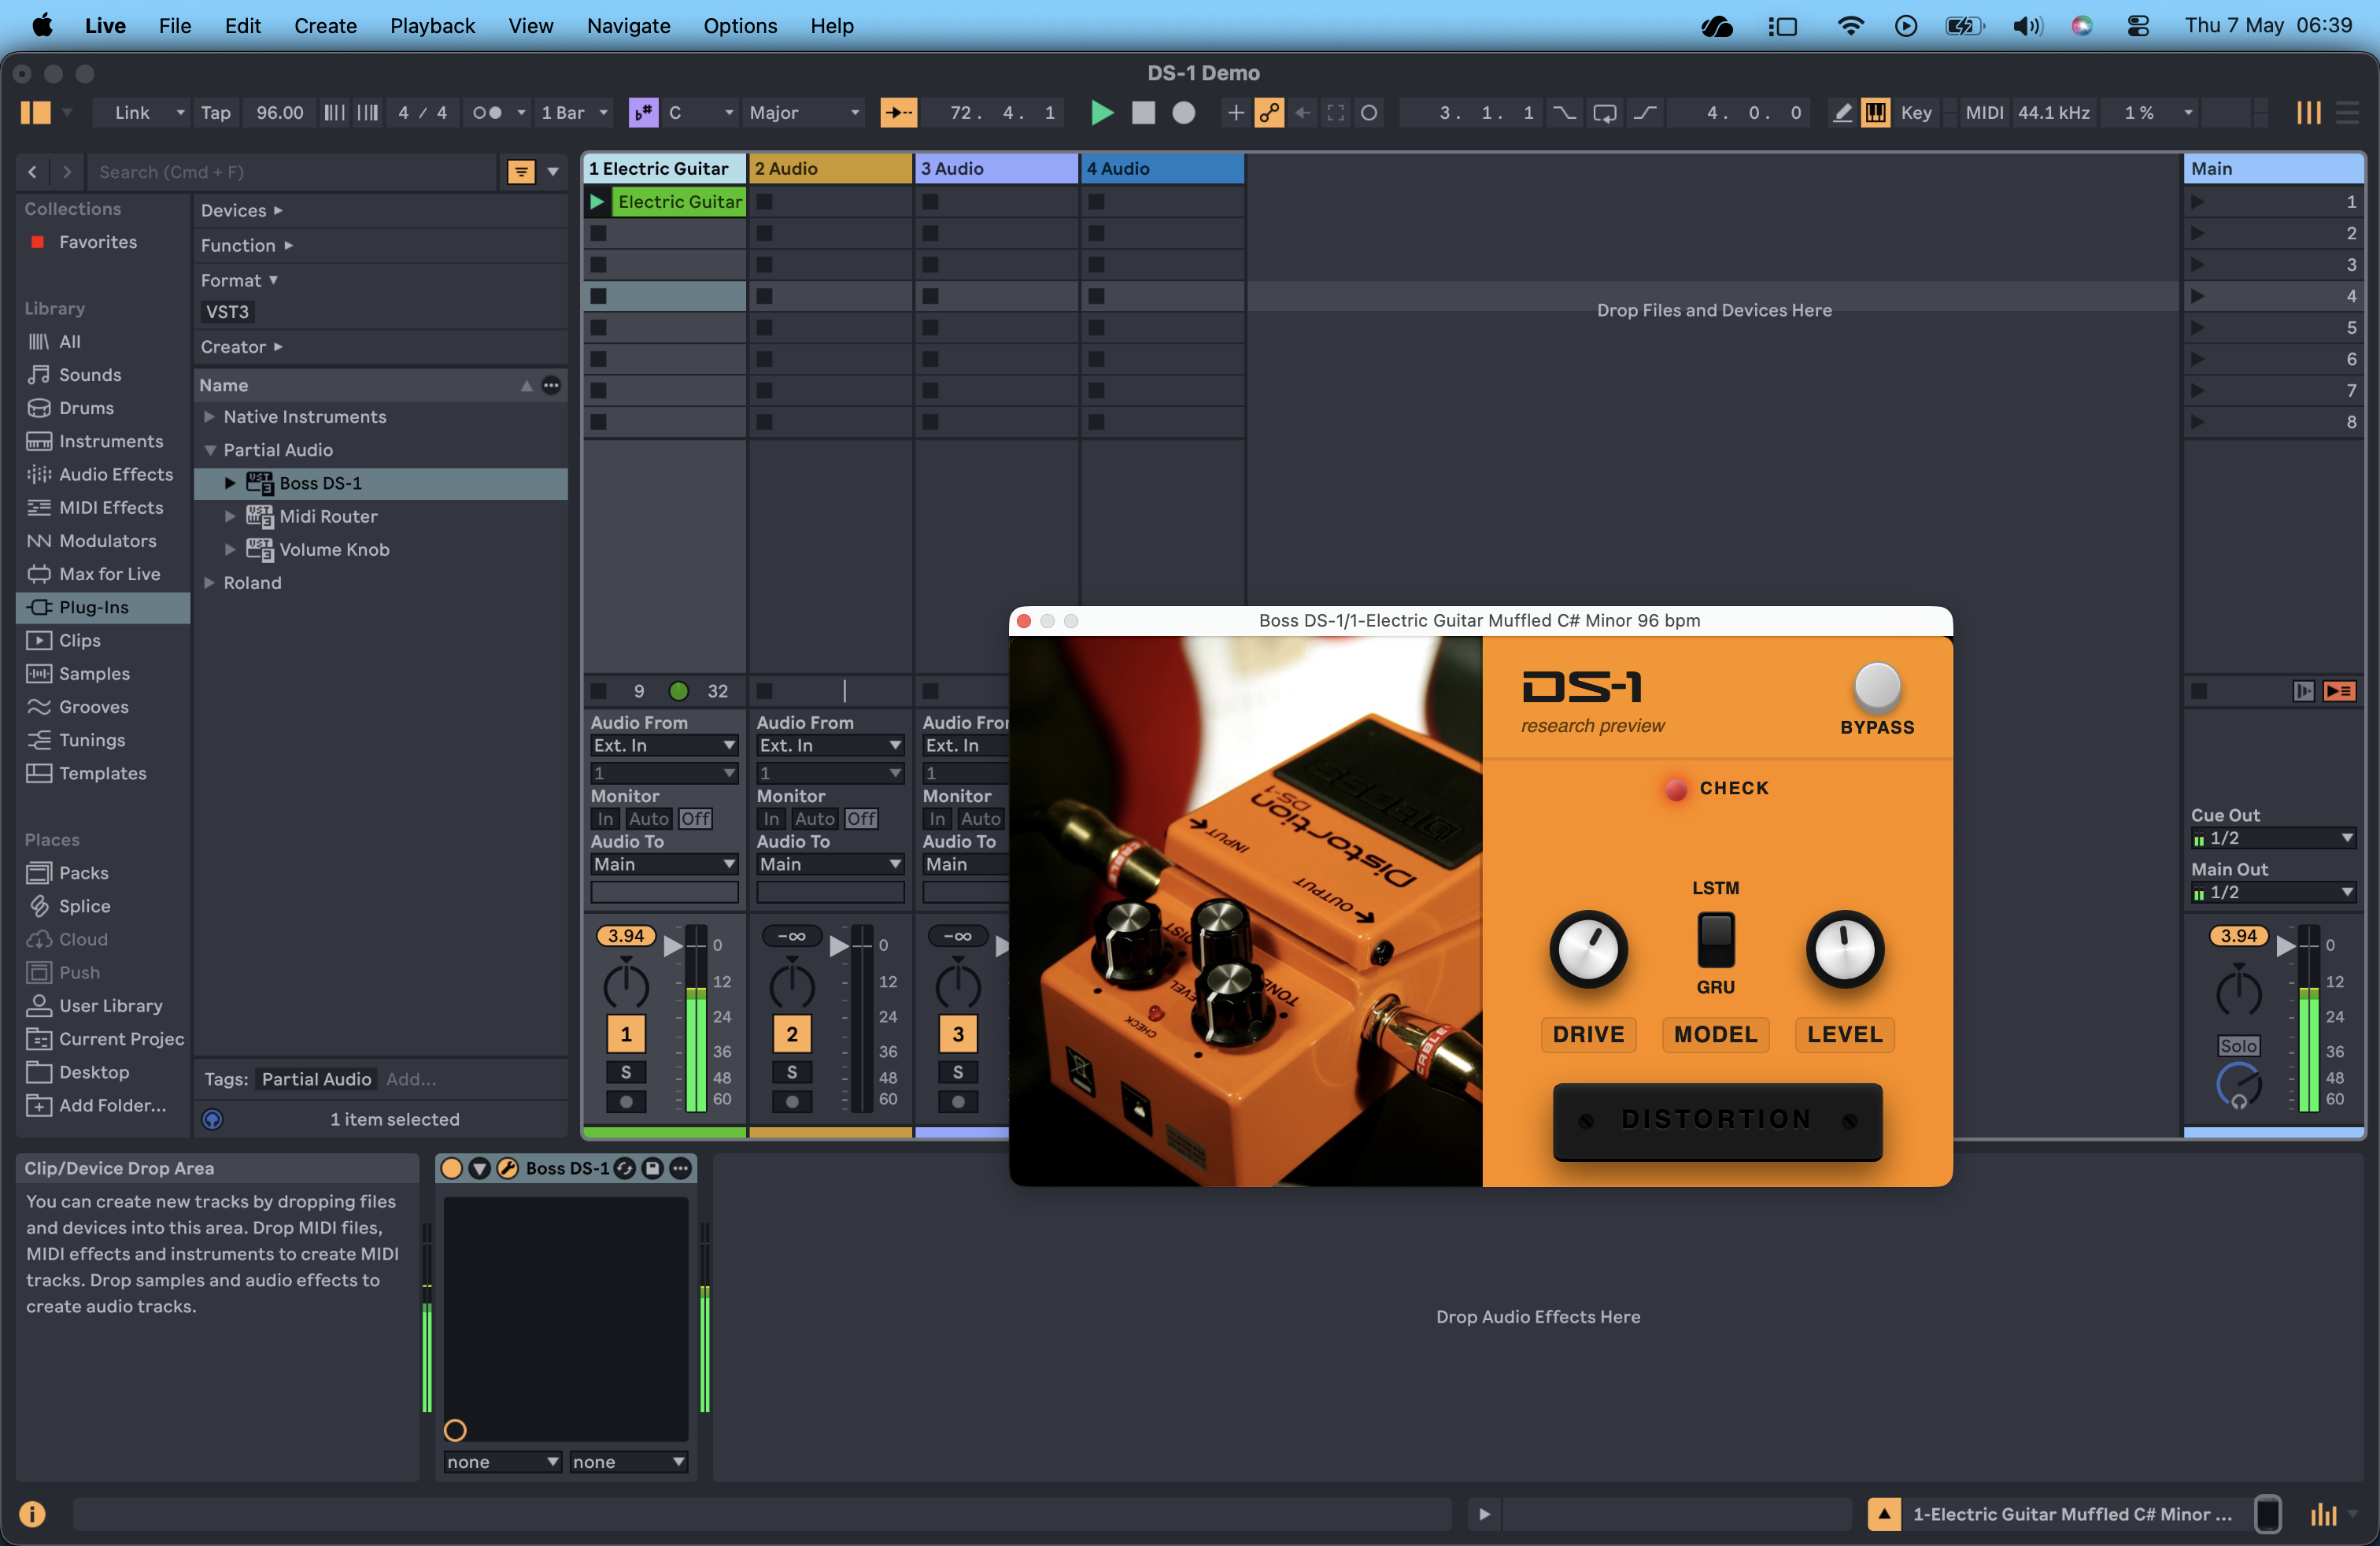
\includegraphics[width=0.9\textwidth]{images/plugin_ui_ableton.png}
  \caption[Plugin interface in Ableton Live 12]{Boss DS-1 neural emulation plugin loaded in Ableton Live 12 during final runtime testing.}
  \label{fig:plugin-ui-ableton-results}
\end{figure}

Model switching between LSTM and GRU behaved correctly in the tested hosts. The hidden state was reset on switching, and no switching artefacts appeared in the reported tests.

No formal CPU benchmark was completed, so this chapter does not report a measured CPU percentage or computational load figure. Inference ran sample-by-sample inside the host audio callback, with no explicit look-ahead or extra buffering stage, so the plugin did not introduce additional algorithmic latency. That should not be read as a measured end-to-end latency benchmark.

\section{Summary of Results}
\label{sec:summary-of-results}

The two architectures separate clearly under the matched hidden-size-24 configuration. The LSTM produced the lower held-out test ESR, along with lower RMSE and MAE, higher error-relative SNR, and higher waveform correlation. The GRU used fewer parameters and stopped much earlier in training, but its validation and test-set error stayed higher.

The exported JSON artefacts loaded into the JUCE and RTNeural plugin, and the plugin operated correctly in the tested VST3 and AU host environments. Drive, Level, Bypass, and Model switching all behaved as expected, with no switching or knob-movement artefacts in the final tests. No formal CPU benchmark was completed, though, and validation did not extend beyond 44.1~kHz host sessions because the non-44.1~kHz resampling path was not part of the tested deployment.

Taken together, the LSTM gave the stronger objective emulation accuracy and the GRU gave the smaller model. The deployed prototype was functionally validated in 44.1~kHz host sessions; formal CPU benchmarking and multi-sample-rate validation remain future work. Chapter 5 picks up this accuracy-efficiency trade-off against the research question, the hidden-size-24 constraint, and the practical demands of real-time neural audio plugin deployment.
